\chapter{Methods}

This chapter will outline the methods how SCVAEs and non-conditioned VAEs are
integrated using multitask learning in this thesis, which will be explored in
the context of images. The chapter will be divided in three sections. The first
section will describe the conditioning strategies, which will be used to
condition the VAEs. In the following section, I will describe the method of
merging SCVAEs with non-conditioned VAEs using two decoders, where one is
conditioned, and the other is not. This method will be referred to as
\method{1}. In the following section, I describe another method of merging
SCVAEs with non-conditioned VAEs by utilizing the same encoder and decoder for
both models by employing novel training strategies, which will be referred to
as \method{2}. Both methods will be applied to both Gaussian VAEs and VQ-VAEs.

\section{Conditioning information}

In this thesis, I will obtain the conditioning information $m$ from the input
image $x$ by sampling pixels some pixels from the input image $x$. In this
process first the first step is to obtain a mask which will be used to sample
the pixels from the input image $x$. The mask will be a binary matrix of the
same size as the input image $x$, where a value of 1 represents the sampled
pixels and a value of 0 represents the pixels that are not sampled. The
decision how many pixels to sample and which pixels to sample will be described
in the following sections for each method.

After the mask is obtained, the mask is applied to the input image $x$ to
obtain the masked image, which is then used to obtain the conditioning
information $m$ by concatenating the mask with the masked image, which can be
seen in Figure~\ref{ConditioningFigure}.

In both proposed methods, the conditioning information $m$ will be incorporated
into decoder by first flattening it and then concatenating it with the input of the decoder and then using a fully connected layer before passing it through the transposed convolutional layers of the decoder.

\begin{figure}
    \centering
    \tikzset{every picture/.style={line width=0.75pt}} %set default line width to 0.75pt        

\begin{tikzpicture}[x=0.75pt,y=0.75pt,yscale=-1,xscale=1]
%uncomment if require: \path (0,300); %set diagram left start at 0, and has height of 300

%Image [id:dp8071272108239995] 
\draw (189,81.67) node  {\includegraphics[width=52.5pt,height=52.5pt]{figures/assets/ORIGINAL_GAUSSIAN.png}};
%Image [id:dp988855448482646] 
\draw (188.33,176) node  {\includegraphics[width=52.5pt,height=52.5pt]{figures/assets/MASK_GAUSSIAN.png}};
%Image [id:dp22673392822113958] 
\draw (309.67,103.67) node  {\includegraphics[width=52.5pt,height=52.5pt]{figures/assets/RESULT_GAUSSIAN.png}};
%Curve Lines [id:da7064061111049843] 
\draw    (224.33,86.33) .. controls (257.99,82.37) and (227.62,107.16) .. (272.29,100.54) ;
\draw [shift={(273.67,100.33)}, rotate = 171.07] [color={rgb, 255:red, 0; green, 0; blue, 0 }  ][line width=0.75]    (10.93,-3.29) .. controls (6.95,-1.4) and (3.31,-0.3) .. (0,0) .. controls (3.31,0.3) and (6.95,1.4) .. (10.93,3.29)   ;
%Curve Lines [id:da2412457613293979] 
\draw    (224.33,157.67) .. controls (273.83,153.05) and (228.59,124.9) .. (272.96,117.23) ;
\draw [shift={(274.33,117)}, rotate = 171.07] [color={rgb, 255:red, 0; green, 0; blue, 0 }  ][line width=0.75]    (10.93,-3.29) .. controls (6.95,-1.4) and (3.31,-0.3) .. (0,0) .. controls (3.31,0.3) and (6.95,1.4) .. (10.93,3.29)   ;
%Image [id:dp7901210362437346] 
\draw (431,111.33) node  {\includegraphics[width=52.5pt,height=52.5pt]{figures/assets/GREEN_GAUSSIAN.png}};
%Image [id:dp9948313666469564] 
\draw (423.67,123) node  {\includegraphics[width=52.5pt,height=52.5pt]{figures/assets/RED_GAUSSIAN.png}};
%Shape: Square [id:dp655934035728707] 
\draw  [color={rgb, 255:red, 255; green, 255; blue, 255 }  ,draw opacity=1 ] (388.67,88) -- (458.67,88) -- (458.67,158) -- (388.67,158) -- cycle ;
%Image [id:dp29091288526835224] 
\draw (417,136) node  {\includegraphics[width=52.5pt,height=52.5pt]{figures/assets/BLUE_GAUSSIAN.png}};
%Shape: Square [id:dp17919766367981604] 
\draw  [color={rgb, 255:red, 255; green, 255; blue, 255 }  ,draw opacity=1 ] (382,101) -- (452,101) -- (452,171) -- (382,171) -- cycle ;
%Image [id:dp6261788477655241] 
\draw (411,148.67) node  {\includegraphics[width=52.5pt,height=52.5pt]{figures/assets/MASK_GAUSSIAN.png}};
%Shape: Square [id:dp8527153376534193] 
\draw  [color={rgb, 255:red, 255; green, 255; blue, 255 }  ,draw opacity=1 ] (376,113.67) -- (446,113.67) -- (446,183.67) -- (376,183.67) -- cycle ;
%Curve Lines [id:da0011889641265926398] 
\draw    (345.67,104.33) .. controls (353.15,122.41) and (361.21,123.58) .. (369.86,125.84) ;
\draw [shift={(371.67,126.33)}, rotate = 195.95] [color={rgb, 255:red, 0; green, 0; blue, 0 }  ][line width=0.75]    (10.93,-3.29) .. controls (6.95,-1.4) and (3.31,-0.3) .. (0,0) .. controls (3.31,0.3) and (6.95,1.4) .. (10.93,3.29)   ;
%Curve Lines [id:da5210657288496086] 
\draw    (224.33,169.67) .. controls (267.89,153.83) and (323.87,157.59) .. (372.2,149.26) ;
\draw [shift={(373.67,149)}, rotate = 169.9] [color={rgb, 255:red, 0; green, 0; blue, 0 }  ][line width=0.75]    (10.93,-3.29) .. controls (6.95,-1.4) and (3.31,-0.3) .. (0,0) .. controls (3.31,0.3) and (6.95,1.4) .. (10.93,3.29)   ;

% Text Node
\draw (162,27.33) node [anchor=north west][inner sep=0.75pt]   [align=left] {Original};
% Text Node
\draw (168.67,123.33) node [anchor=north west][inner sep=0.75pt]   [align=left] {Mask};
% Text Node
\draw (420.67,50.67) node [anchor=north west][inner sep=0.75pt]   [align=left] {$\displaystyle m$};


\end{tikzpicture}

    \caption[The illustration of the process of obtaining the conditioning information $m$ from the input image $x$ and the mask.]%
    {
        The illustration of the process of obtaining the conditioning information $m$ from the input image $x$ and the mask. The process to obtain the conditioning information $m$ consists of two steps: the first step is to obtain the masked image from the input image $x$ and the mask, and the second step is to add the mask to the masked image to obtain the conditioning information $m$. The conditioning information $m$ is then used to condition the decoder.
    }\label{ConditioningFigure}
\end{figure}

\section{\method{1}}

In the first method, VAEs framework is expanded with a second decoder
$p_\xi(x|z,m)$, which is conditioned on an additional property $m$ of the input
data. This approach involves utilizing two decoders within the VAEs framework:
one for reconstructing the input data solely based on the latent variable $z$,
and the other for reconstructing the input data based on both the latent
variable $z$ and the additional conditioning information $m$.

\subsection{Conditioning strategy}

In this method, the conditioning information $m$ is acquired by sampling
constant number of pixels from the input data. To sample the pixels from the
input image $x$, I will use a pixel sampling operation, which will be described
in the following section.

\subsubsection{Pixel Sampling operation}

I will explore two pixel sampling types for this method,
which can be seen in Figure~\ref{SamplingFigure} and are described as follows:

\begin{enumerate}
    \item \textbf{Exact same sampling:} In this sampling type, the conditioning information $m$ is sampled from the input image $x$ by sampling the exact same sparse pixels from the input image $x$. In this work, the pixels that will be sampled from the input image will be a sparse grid of pixels.
    \item \textbf{Uniform random sampling:} In this sampling type, the conditioning information $m$ is sampled from the input image $x$ by sampling exact number of pixels from the input image $x$ uniformly at random.
\end{enumerate}

The sampling process will be done every time the input image $x$ is passed through the model. This means that in the case of the uniform random sampling, the conditioning information $m$ will be different for each time the image is passed through the model. This is done to ensure that the model learns to generalize and handle various cases.

\subsection{Application to Gaussian VAEs}

In Gaussian VAEs, the integration of a second conditioned decoder
$p_\xi(x|z,m)$ follows a similar approach as outlined in the general method
description. However, there are specific adjustments and considerations that
need to be taken into account when applying this method to Gaussian VAEs.

The integration of the second conditioned decoder $p_\xi(x|z,m)$ into the
Gaussian VAEs framework involves flattening on concatenating the latent
variable $z$ and the conditioning information $m$ and passing it through a
fully connected layer before passing it through the transposed convolutional
layers of the second decoder. Although a new latent variable could have
been sampled for the second decoder, the same latent variable $z$ is used
instead of sampling a new one. This is done to ensure that the latent variable
$z$ is the same for both decoders and ensure that it is easier to compare the
reconstructions of the input data. The architecture of the Gaussian
VAEs framework with the second conditioned decoder is illustrated in
Figure~\ref{SCVAE2DFigure}

Although the training strategy could have been to train decoders by alternating between them, in this thesis, I will explore the training strategy where both decoders are trained simultaneously.

In Gaussian VAEs, the loss objective consists of two components: the
reconstruction loss and the KL divergence term. However, with the inclusion of
the second conditioned decoder, the loss objective is extended to include the
reconstruction loss of the second conditioned decoder. The overall loss
objective to be \textbf{minimized} becomes

\[ L = W_1 \frac{1}{D} \sum_{i=1}^{D} ||x_i - \hat{x}_{1_{i}} ||^2 + W_2 \frac{1}{D} \sum_{i=1}^{D} || x_i - \hat{x}_{2_{i}} ||^2 + \beta  \frac{1}{2} \sum_{i=1}^{Z} \biggl( -\log \sigma^2_\phi(x)_i - 1 + \mu^2_\phi(x)_i + \sigma^2_\phi(x)_i \biggr), \]

where $D$ is the number of pixels in the input image, $x_i$ is the $i$-th pixel
of the input image, $\hat{x}_1$ is the output of the first decoder, $\hat{x}_2$
is the output of the second decoder, $\beta$ is the KL divergence weight, Z is
the dimension of the latent space, $\mu_\phi(x)$ and $\sigma_\phi(x)$ are the
mean and the standard deviation of the Gaussian distribution produced by the
encoder, respectively. The resulting loss has also extra weight parameters $W_1$ and $W_2$ to balance and control the importance of reconstruction loss, which will be hyperparameters of the model.

During the training process, the encoder is trained to produce accurate mean
and standard deviation of the Gaussian distribution, and the decoders are
trained to produce accurate reconstructions of the input data. The KL
divergence term is used to regularize the latent space to be close to a
standard Gaussian distribution. The optimizer used to minimize the overall loss
objective is the AdamW optimizer~\cite{AdamW}.

As a result of the integration of the second conditioned decoder, the model has
the ability to reconstruct the input data based just on the latent variable $z$
and as well as the conditioning information $m$.
\begin{figure}[H]
    \centering
    

\tikzset{every picture/.style={line width=0.75pt}} %set default line width to 0.75pt        

\begin{tikzpicture}[x=0.75pt,y=0.75pt,yscale=-1,xscale=1]
%uncomment if require: \path (0,348); %set diagram left start at 0, and has height of 348

%Shape: Trapezoid [id:dp934357521829376] 
\draw  [fill={rgb, 255:red, 245; green, 166; blue, 35 }  ,fill opacity=1 ] (108.26,123.49) -- (210.56,161.61) -- (210.56,204.73) -- (108.26,242.84) -- cycle ;
%Flowchart: Alternative Process [id:dp9932499259340365] 
\draw  [color={rgb, 255:red, 208; green, 2; blue, 27 }  ,draw opacity=1 ][dash pattern={on 4.5pt off 4.5pt}] (328.6,122.37) .. controls (340.2,122.37) and (349.6,131.77) .. (349.6,143.37) -- (349.6,221.37) .. controls (349.6,232.96) and (340.2,242.37) .. (328.6,242.37) -- (250.6,242.37) .. controls (239,242.37) and (229.6,232.96) .. (229.6,221.37) -- (229.6,143.37) .. controls (229.6,131.77) and (239,122.37) .. (250.6,122.37) -- cycle ;
%Shape: Trapezoid [id:dp09230270953752695] 
\draw  [fill={rgb, 255:red, 245; green, 166; blue, 35 }  ,fill opacity=1 ] (472.3,306.92) -- (370,268.8) -- (370,225.68) -- (472.3,187.57) -- cycle ;
%Straight Lines [id:da8721986267989312] 
\draw    (86,183.92) -- (106.33,183.69) ;
\draw [shift={(108.33,183.67)}, rotate = 179.36] [color={rgb, 255:red, 0; green, 0; blue, 0 }  ][line width=0.75]    (10.93,-3.29) .. controls (6.95,-1.4) and (3.31,-0.3) .. (0,0) .. controls (3.31,0.3) and (6.95,1.4) .. (10.93,3.29)   ;
%Straight Lines [id:da04043808992603615] 
\draw    (156,244.83) -- (156,226.17) ;
\draw [shift={(156,224.17)}, rotate = 90] [color={rgb, 255:red, 0; green, 0; blue, 0 }  ][line width=0.75]    (10.93,-3.29) .. controls (6.95,-1.4) and (3.31,-0.3) .. (0,0) .. controls (3.31,0.3) and (6.95,1.4) .. (10.93,3.29)   ;
%Straight Lines [id:da7995820072131101] 
\draw    (470.53,250.33) -- (483,250.19) ;
\draw [shift={(485,250.17)}, rotate = 179.34] [color={rgb, 255:red, 0; green, 0; blue, 0 }  ][line width=0.75]    (10.93,-3.29) .. controls (6.95,-1.4) and (3.31,-0.3) .. (0,0) .. controls (3.31,0.3) and (6.95,1.4) .. (10.93,3.29)   ;
%Straight Lines [id:da04854862230740742] 
\draw    (418.03,304.8) -- (418.03,288.8) ;
\draw [shift={(418.03,286.8)}, rotate = 90] [color={rgb, 255:red, 0; green, 0; blue, 0 }  ][line width=0.75]    (10.93,-3.29) .. controls (6.95,-1.4) and (3.31,-0.3) .. (0,0) .. controls (3.31,0.3) and (6.95,1.4) .. (10.93,3.29)   ;
%Straight Lines [id:da28655754211367357] 
\draw    (264.67,148.01) -- (281.6,148.01) ;
%Straight Lines [id:da8743242231946385] 
\draw    (264,183.17) -- (281.6,183.17) ;
%Straight Lines [id:da7034471264471225] 
\draw    (281.6,148.01) -- (281.6,183.17) ;
%Straight Lines [id:da513676610842577] 
\draw    (300.67,218.15) -- (265.33,218.15) ;
%Straight Lines [id:da6342992244346165] 
\draw    (300.67,161.61) -- (300.67,218.15) ;
%Straight Lines [id:da9216809508784987] 
\draw    (295.33,161.61) -- (300.67,161.61) ;
%Straight Lines [id:da7099642706169568] 
\draw    (300.67,183.17) -- (311.33,183.17) ;
\draw [shift={(313.33,183.17)}, rotate = 180] [color={rgb, 255:red, 0; green, 0; blue, 0 }  ][line width=0.75]    (10.93,-3.29) .. controls (6.95,-1.4) and (3.31,-0.3) .. (0,0) .. controls (3.31,0.3) and (6.95,1.4) .. (10.93,3.29)   ;
%Straight Lines [id:da7247942827107159] 
\draw    (210,183.17) -- (234,183.17) ;
\draw [shift={(236,183.17)}, rotate = 180] [color={rgb, 255:red, 0; green, 0; blue, 0 }  ][line width=0.75]    (10.93,-3.29) .. controls (6.95,-1.4) and (3.31,-0.3) .. (0,0) .. controls (3.31,0.3) and (6.95,1.4) .. (10.93,3.29)   ;
%Straight Lines [id:da63134479510402] 
\draw    (210,183.17) -- (236.1,216.57) ;
\draw [shift={(237.33,218.15)}, rotate = 232] [color={rgb, 255:red, 0; green, 0; blue, 0 }  ][line width=0.75]    (10.93,-3.29) .. controls (6.95,-1.4) and (3.31,-0.3) .. (0,0) .. controls (3.31,0.3) and (6.95,1.4) .. (10.93,3.29)   ;
%Shape: Trapezoid [id:dp8668843769015238] 
\draw  [fill={rgb, 255:red, 245; green, 166; blue, 35 }  ,fill opacity=1 ] (472.3,175.97) -- (370,137.85) -- (370,94.73) -- (472.3,56.62) -- cycle ;
%Straight Lines [id:da2460263598329412] 
\draw    (472.33,118.57) -- (481.67,118.57) ;
\draw [shift={(483.67,118.57)}, rotate = 180] [color={rgb, 255:red, 0; green, 0; blue, 0 }  ][line width=0.75]    (10.93,-3.29) .. controls (6.95,-1.4) and (3.31,-0.3) .. (0,0) .. controls (3.31,0.3) and (6.95,1.4) .. (10.93,3.29)   ;
%Curve Lines [id:da14884210290991218] 
\draw    (330,168.67) .. controls (343.79,141.55) and (331.38,133.09) .. (368.28,119.2) ;
\draw [shift={(370,118.57)}, rotate = 159.91] [color={rgb, 255:red, 0; green, 0; blue, 0 }  ][line width=0.75]    (10.93,-3.29) .. controls (6.95,-1.4) and (3.31,-0.3) .. (0,0) .. controls (3.31,0.3) and (6.95,1.4) .. (10.93,3.29)   ;
%Curve Lines [id:da337205815747899] 
\draw    (329,196.67) .. controls (338.85,230.62) and (332.53,236.66) .. (368.33,249.28) ;
\draw [shift={(370,249.87)}, rotate = 199.09] [color={rgb, 255:red, 0; green, 0; blue, 0 }  ][line width=0.75]    (10.93,-3.29) .. controls (6.95,-1.4) and (3.31,-0.3) .. (0,0) .. controls (3.31,0.3) and (6.95,1.4) .. (10.93,3.29)   ;
%Rounded Rect [id:dp043688298303683815] 
\draw  [fill={rgb, 255:red, 248; green, 231; blue, 28 }  ,fill opacity=1 ] (158,72.37) .. controls (158,67.56) and (161.9,63.67) .. (166.7,63.67) -- (241.3,63.67) .. controls (246.1,63.67) and (250,67.56) .. (250,72.37) -- (250,98.47) .. controls (250,103.27) and (246.1,107.17) .. (241.3,107.17) -- (166.7,107.17) .. controls (161.9,107.17) and (158,103.27) .. (158,98.47) -- cycle ;
%Curve Lines [id:da2856571407609658] 
\draw    (61,139.5) .. controls (69.87,73.5) and (119.48,87.23) .. (157.28,82.88) ;
\draw [shift={(159,82.67)}, rotate = 172.5] [color={rgb, 255:red, 0; green, 0; blue, 0 }  ][line width=0.75]    (10.93,-3.29) .. controls (6.95,-1.4) and (3.31,-0.3) .. (0,0) .. controls (3.31,0.3) and (6.95,1.4) .. (10.93,3.29)   ;
%Curve Lines [id:da22903393349913204] 
\draw    (290,84.67) .. controls (332.79,82.68) and (295.38,106.43) .. (368.88,108.64) ;
\draw [shift={(370,108.67)}, rotate = 181.53] [color={rgb, 255:red, 0; green, 0; blue, 0 }  ][line width=0.75]    (10.93,-3.29) .. controls (6.95,-1.4) and (3.31,-0.3) .. (0,0) .. controls (3.31,0.3) and (6.95,1.4) .. (10.93,3.29)   ;
%Straight Lines [id:da009477353404151012] 
\draw    (412,168.67) -- (412,154.67) ;
\draw [shift={(412,152.67)}, rotate = 90] [color={rgb, 255:red, 0; green, 0; blue, 0 }  ][line width=0.75]    (10.93,-3.29) .. controls (6.95,-1.4) and (3.31,-0.3) .. (0,0) .. controls (3.31,0.3) and (6.95,1.4) .. (10.93,3.29)   ;
%Straight Lines [id:da9811464459973317] 
\draw    (250,86.67) -- (260.01,85.83) ;
\draw [shift={(262,85.67)}, rotate = 175.24] [color={rgb, 255:red, 0; green, 0; blue, 0 }  ][line width=0.75]    (10.93,-3.29) .. controls (6.95,-1.4) and (3.31,-0.3) .. (0,0) .. controls (3.31,0.3) and (6.95,1.4) .. (10.93,3.29)   ;
%Image [id:dp9476502325775372] 
\draw (61,175) node  {\includegraphics[width=52.5pt,height=52.5pt]{figures/assets/SCVAE2D_16/original.png}};
%Image [id:dp2988278977003932] 
\draw (520,249) node  {\includegraphics[width=52.5pt,height=52.5pt]{figures/assets/SCVAE2D_16/non-conditioned-decoder-output.png}};
%Image [id:dp02921342288140205] 
\draw (519,110) node  {\includegraphics[width=52.5pt,height=52.5pt]{figures/assets/SCVAE2D_16/condiotioned-decoder-output.png}};

% Text Node
\draw (129.67,174.67) node [anchor=north west][inner sep=0.75pt]   [align=left] {Encoder};
% Text Node
\draw (392.8,239.87) node [anchor=north west][inner sep=0.75pt]   [align=left] {Decoder$\displaystyle _{1}$};
% Text Node
\draw  [fill={rgb, 255:red, 248; green, 231; blue, 28 }  ,fill opacity=1 ]  (155.17, 258.5) circle [x radius= 13.9, y radius= 13.9]   ;
\draw (148.67,250.9) node [anchor=north west][inner sep=0.75pt]    {$\phi $};
% Text Node
\draw  [fill={rgb, 255:red, 208; green, 2; blue, 27 }  ,fill opacity=0.49 ]  (250.6, 148.01) circle [x radius= 13.6, y radius= 13.6]   ;
\draw (244.6,140.41) node [anchor=north west][inner sep=0.75pt]    {$\epsilon $};
% Text Node
\draw  [fill={rgb, 255:red, 248; green, 231; blue, 28 }  ,fill opacity=1 ]  (416.83, 319) circle [x radius= 13.6, y radius= 13.6]   ;
\draw (410.83,311.4) node [anchor=north west][inner sep=0.75pt]    {$\theta $};
% Text Node
\draw  [fill={rgb, 255:red, 155; green, 155; blue, 155 }  ,fill opacity=0.3 ]  (250.6, 182.17) circle [x radius= 13.6, y radius= 13.6]   ;
\draw (244.6,174.57) node [anchor=north west][inner sep=0.75pt]    {$\sigma $};
% Text Node
\draw  [fill={rgb, 255:red, 155; green, 155; blue, 155 }  ,fill opacity=0.3 ]  (250.6, 218.15) circle [x radius= 13.6, y radius= 13.6]   ;
\draw (244.6,210.55) node [anchor=north west][inner sep=0.75pt]    {$\mu $};
% Text Node
\draw  [fill={rgb, 255:red, 155; green, 155; blue, 155 }  ,fill opacity=0.3 ]  (326.6, 183.17) circle [x radius= 13.6, y radius= 13.6]   ;
\draw (320.6,175.57) node [anchor=north west][inner sep=0.75pt]    {$z$};
% Text Node
\draw (279.67,152.01) node [anchor=north west][inner sep=0.75pt]    {$\odot $};
% Text Node
\draw (263.67,102.17) node [anchor=north west][inner sep=0.75pt]  [color={rgb, 255:red, 208; green, 2; blue, 27 }  ,opacity=1 ] [align=left] {{\tiny Reparam. trick}};
% Text Node
\draw (392.8,108.57) node [anchor=north west][inner sep=0.75pt]   [align=left] {Decoder$\displaystyle _{2}$};
% Text Node
\draw (173,75.17) node [anchor=north west][inner sep=0.75pt]   [align=left] {Sampling};
% Text Node
\draw  [fill={rgb, 255:red, 248; green, 231; blue, 28 }  ,fill opacity=1 ]  (412.83, 183.17) circle [x radius= 13.6, y radius= 13.6]   ;
\draw (406.83,175.57) node [anchor=north west][inner sep=0.75pt]    {$\xi $};
% Text Node
\draw  [fill={rgb, 255:red, 155; green, 155; blue, 155 }  ,fill opacity=0.3 ]  (276.1, 84.17) circle [x radius= 14.53, y radius= 14.53]   ;
\draw (268.6,76.57) node [anchor=north west][inner sep=0.75pt]    {$m$};


\end{tikzpicture}

    \caption[\method{1} applied to Gaussian VAEs.]%
    {
        \methodOne\ applied to Gaussian VAEs. The Gaussian VAEs framework is extended by adding a second conditioned decoder $p_\xi(x|z,m)$. The input $x$ is passed through the encoder with parameters $\phi$ producing the mean $\mu$ and the standard deviation $\sigma$ of the Gaussian distribution. The random variable $\epsilon$ is sampled from a standard Gaussian distribution and is used to sample $ z = \mu + \sigma \odot \epsilon$. The sampled $z$ is then used as input to both decoders. As a result, the loss function consists of three components: the MSE reconstruction loss of the first decoder, the MSE reconstruction loss of the second decoder and the KL divergence regularization loss.
    }\label{SCVAE2DFigure}
\end{figure}

\subsection{Application to VQ-VAEs}

The approach of integrating the second conditioned decoder $p_\xi(x|z,m)$ into
the VQ-VAEs framework is similar to the approach used for Gaussian VAEs.
However, there differences that need to be taken into account when applying
this method to VQ-VAEs.

One of the main differences is that the VQ-VAEs framework uses a discrete
latent space and the Vector Quantization which is described in \autoref{background:vqvae}. This means that the latent variable $z$ is a discrete variable which represents the indexes of the embedding table vectors. This means that first the corresponding embedding table vectors $z_q(x)$ must be computed for the latent variable $z$ before flattening and concatenating it with the conditioning information $m$ and then using a fully connected layer before the transposed convolutional layers of the second decoder. The architecture of the VQ-VAEs framework with the second conditioned decoder is illustrated in Figure~\ref{SCVQVAE2DFigure}.

The training strategy is the same as in Gaussian VAEs, where both decoders are trained simultaneously. This means that the loss objective must be extended to include the reconstruction loss of the second conditioned decoder. In VQ-VAEs, the loss objective consists of three components: the MSE
reconstruction loss and the commitment loss and the codebook loss. However,
with the inclusion of the second conditioned decoder, the loss objective is
extended to include the reconstruction loss of the second conditioned decoder.
The overall loss objective to be \textbf{minimized} becomes

\[ L = W_1 \frac{1}{D} \sum_{i=1}^{D} ||x_i - \hat{x}_{1_{i}} ||^2 +  W_2 \frac{1}{D} \sum_{i=1}^{D} || x_i - \hat{x}_{2_{i}} ||^2 + \frac{1}{Z} \sum_{i=1}^{Z} \biggl( || sg(z_e(x)_i) - e_{k_i} ||^2 + \beta || z_q(x)_i - sg(e_{k{_i}}) ||^2 \biggr) , \]

% TODO explain the weights W1 and W2

where $D$ is the number of pixels in the input image, $x_i$ is the $i$-th pixel
of the input image, $\hat{x}_1$ is the output of the first decoder, $\hat{x}_2$
is the output of the second decoder, $Z$ is the number of latent space vectors,
$z_e(x)$ is the output of the encoder, $z_q(x)$ is the mapping output after
Vector Quantization, $e_k$ is the $k$-th embedding table vector, $\beta$ is the
commitment loss weight, $sg$ is the stop gradient operation, which was
previously defined in the background \autoref{background:vqvae}.

After the first stage of the training, the model has the ability to reconstruct
the input data based just on the latent variable $z$ and as well as the
conditioning information $m$. To generate the latent variable $z$ there must be
trained a separate autoregressive model, which will be used to generate the
latent variable $z$.

\begin{figure}[H]
    \centering
    \centering
\scriptsize
\begin{tabular}{||c|c|c|c||}
\hline
 Method & Parameters & Reconstruction loss & KL loss \\
\hline
\textit{Baseline} & - & 0.0089 +- 2.2e-06 & 0.0074 +- 6.6e-06 \\
\hline
Multi Decoder & Exact sampling & 0.0064 +- 6.5e-07  $\downarrow$ & 0.0088 +- 3.1e-06  $\uparrow$ \\
\hline
Multi Decoder & Exact sampling, SoftAdapt & 0.0292 +- 7.4e-04  $\uparrow$ & 0.0031 +- 9.7e-06  $\downarrow$ \\
\hline
Multi Decoder & Uniform sampling & 0.0063 +- 6.1e-08  $\downarrow$ & 0.0099 +- 4.0e-07  $\uparrow$ \\
\hline
Multi Decoder & Uniform sampling, SoftAdapt & 0.0277 +- 4.5e-04  $\uparrow$ & 0.0026 +- 6.8e-06  $\downarrow$ \\
\hline
\end{tabular}

    \caption[\method{1} applied to VQ-VAEs.]%
    {
        \method{1} applied to VQ-VAEs. The VQ-VAEs framework is extended by adding a second conditioned decoder. Instead of using a fully connected layer to merge the latent variable $z$ and the conditioning information $m$, the corresponding embedding table vectors $z_q(x)$ must be computed for the latent variable $z$ before merging it with the conditioning information $m$. As a result of adding the second conditioned decoder, the loss function requires the addition of the MSE reconstruction loss of the second decoder.
    }\label{SCVQVAE2DFigure}
\end{figure}

\section{\method{2}}

In the \method{2}, the idea is to employ a single decoder within the VAE architecture that is capable of reconstructing the input data under variable conditioning. The variable conditioning means that the conditioning information $m$ can be a variable amount of information or just an empty mask. This method differs from the \method{1} in that it uses a single decoder for both tasks and dynamically adjusts its behavior based on the amount of information present in the variable $m$.

This method utilizes a single decoder that dynamically adjusts its behavior
based on the amount of information present in the variable $m$. When the
conditioning information is available, the decoder incorporates it into the
reconstruction process and takes advantage of it to get the best
reconstruction. Otherwise, it operates solely based on the latent variable $z$.

To achieve this, in this method I will use different conditioning strategy, which will be described in the following subsection.

\subsection{Conditioning strategy}

Similar to the previous method, the conditioning information $m$ is acquired by
sampling pixels from the input image $x$. However, in this method the process of sampling the conditioning information $m$ is different in that the conditioning information $m$ is sampled by selecting a variable number of pixels from the input image $x$. This is done to ensure that the decoder of the model learns to handle various cases where there is variable conditioning information.

To achieve this, I will implement a two-step sampling process:

\begin{enumerate}
    \item \textbf{Sampling the number of pixels:} In this step, the number of pixels to be sampled from the input image $x$ is sampled from a power law distribution. The power law distribution is scaled to the size of the input image $x$ and is used to sample the number of pixels to be sampled from the input image $x$.
    \item \textbf{Sampling the pixels:} In this step, the conditioning information $m$ is sampled from the input image $x$ by sampling the number of pixels sampled in the previous step from the input image: uniformly at random or from a Gaussian distribution. Both of these sampling types can be seen in Figure~\ref{SamplingFigure}.
\end{enumerate}

The sampling two-step process will be done every time the input image $x$ is passed through the model. This means that the conditioning information $m$ will be different for each time the image is passed through the model. This is done to ensure that the model learns to generalize and handle various cases.

During training, the number of pixels to be sampled from the input image $x$ varies every time the input image $x$ is passed through the model and is sampled from a power law distribution.
The power law distribution is chosen because it can have finite range and scalability, which makes it suitable for sampling the number of pixels from the input image. The exponent of the power law distribution will be chosen to be high so that the decoder can learn to handle also the cases where the conditioning information is not available. The exponent will be a hyperparameter of the model.


\subsection{Application to Gaussian VAEs}

In Gaussian VAEs, applying the second method involves modifying the decoder to
be capable of reconstructing the input data under variable conditioning. The
modified decoder $p_\xi(x|z,m)$ is capable of reconstructing the input data
based on the latent variable $z$ and the conditioning information $m$ or just
the latent variable $z$.

This is achieved by using a fully connected layer to merge the latent variable
$z$ and the conditioning information $m$ before passing it through the
transposed convolutional layers. The architecture of the Gaussian VAEs
framework with a single decoder capable of variable conditioning is illustrated
in Figure~\ref{SCVAE1DFigure}.

\begin{figure}[H]
    \centering
    \centering
\scriptsize
\begin{tabular}{||c|c|c|c||}
\hline
 Method & Parameters & Reconstruction loss & KL loss \\
\hline
\textit{Baseline} & - & 0.0047 +- 3.9e-04 & 0.0015 +- 3.1e-04 \\
\hline
Single Decoder & Gaussian sampling, Exponent=40 & 0.0045 +- 1.4e-03  $\downarrow$ & 0.0012 +- 4.1e-04  $\downarrow$ \\
\hline
Single Decoder & Gaussian sampling, Exponent=60 & 0.0045 +- 2.1e-03  $\downarrow$ & 0.0012 +- 5.9e-04  $\downarrow$ \\
\hline
Single Decoder & Uniform sampling, Exponent=40 & 0.0046 +- 1.2e-03  $\downarrow$ & 0.0012 +- 4.2e-04  $\downarrow$ \\
\hline
Single Decoder & Uniform sampling, Exponent=60 & 0.0046 +- 1.1e-03  $\downarrow$ & 0.0012 +- 1.6e-04  $\downarrow$ \\
\hline
\end{tabular}

    \caption[\method{2} applied to Gaussian VAEs.]%
    {
        \methodTwo\ applied to Gaussian VAEs. The Gaussian VAEs framework is modified by allowing the decoder to be conditioned on a variable amount of information and to dynamically adjust its behavior based on the amount of information present in the variable $m$. The input $x$ is passed through the encoder with parameters $\phi$ producing the mean $\mu$ and the standard deviation $\sigma$ of the Gaussian distribution. The random variable $\epsilon$ is sampled from a standard Gaussian distribution and is used to sample $ z = \mu + \sigma \odot \epsilon$. The sampled $z$ is then used as input to the decoder as well as the extra conditioning information $m$. With this approach there is no need for a second decoder, as the single decoder is capable to reconstruct the data based on the latent variable $z$ and the conditioning information $m$ or just the latent variable $z$.
    }\label{SCVAE1DFigure}
\end{figure}

\subsection{Application to VQ-VAEs}

In VQVAEs, same as in Gaussian VAEs, the second method involves modifying the
decoder to be capable to receive variable conditioning information. Unlike
Gaussian VAEs, the VQ-VAEs use Vector Quantization to discretize the continuous
latent space. Because of this, the latent variable $z$ can not be directly
merged with the conditioning information $m$ using a fully connected layer.
Instead, the corresponding embedding table vectors $z_q(x)$ must be computed
for the latent variable $z$ before merging it with the conditioning information
$m$. The architecture of the VQ-VAEs framework with a single decoder capable of
variable conditioning is illustrated in Figure~\ref{SCVQVAE1DFigure}.

\begin{figure}[H]
    \centering
    

\tikzset{every picture/.style={line width=0.75pt}} %set default line width to 0.75pt        

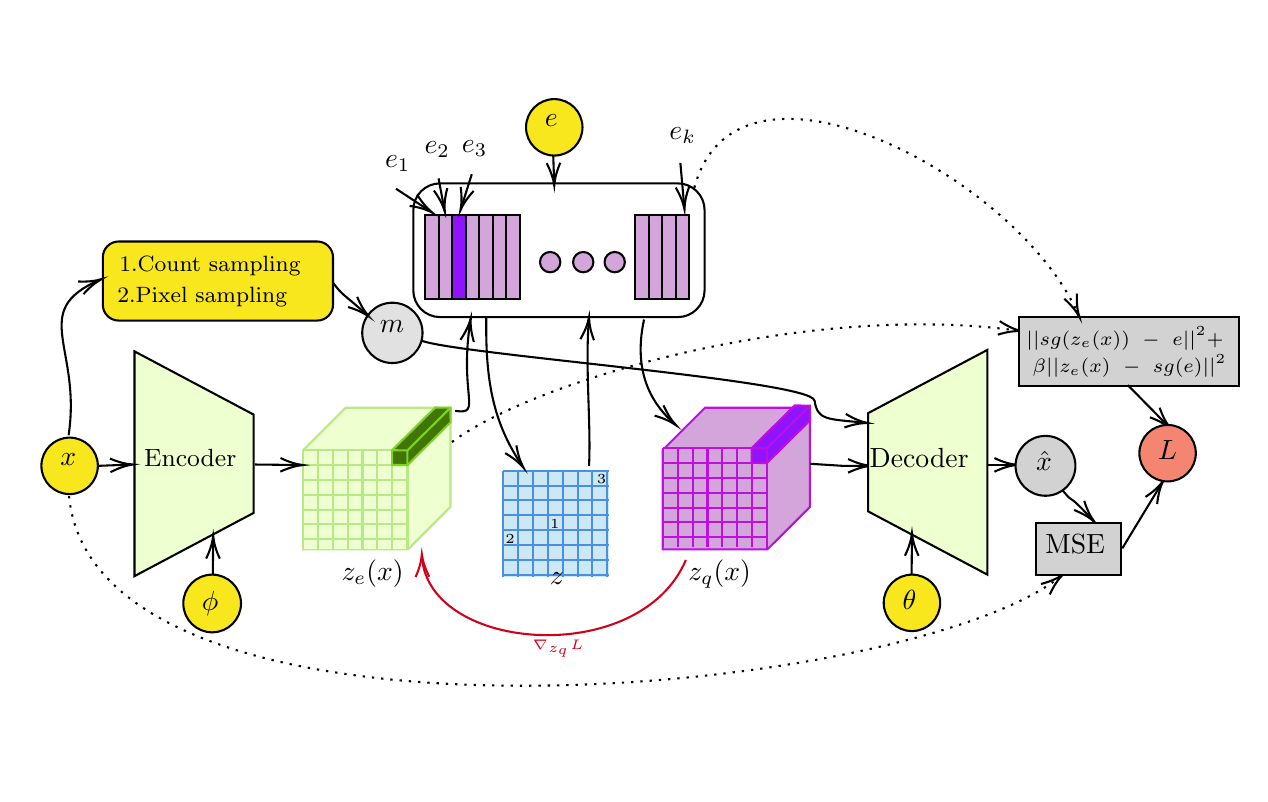
\begin{tikzpicture}[x=0.75pt,y=0.75pt,yscale=-1,xscale=1]
%uncomment if require: \path (0,308); %set diagram left start at 0, and has height of 308

%Shape: Trapezoid [id:dp6171005453979647] 
\draw  [fill={rgb, 255:red, 238; green, 255; blue, 208 }  ,fill opacity=1 ] (107.75,142.44) -- (165.17,172.91) -- (165.17,220.26) -- (107.75,250.73) -- cycle ;
%Shape: Cube [id:dp24555481618180852] 
\draw  [color={rgb, 255:red, 184; green, 233; blue, 134 }  ,draw opacity=1 ][fill={rgb, 255:red, 238; green, 255; blue, 208 }  ,fill opacity=1 ] (189,190.06) -- (209.47,169.59) -- (260,169.59) -- (260,217.36) -- (239.53,237.83) -- (189,237.83) -- cycle ; \draw  [color={rgb, 255:red, 184; green, 233; blue, 134 }  ,draw opacity=1 ] (260,169.59) -- (239.53,190.06) -- (189,190.06) ; \draw  [color={rgb, 255:red, 184; green, 233; blue, 134 }  ,draw opacity=1 ] (239.53,190.06) -- (239.53,237.83) ;
%Shape: Grid [id:dp05381914789010611] 
\draw  [draw opacity=0][fill={rgb, 255:red, 238; green, 255; blue, 208 }  ,fill opacity=1 ][line width=0.75]  (189,190.06) -- (239.36,190.06) -- (239.36,237.83) -- (189,237.83) -- cycle ; \draw  [color={rgb, 255:red, 184; green, 233; blue, 134 }  ,draw opacity=1 ][line width=0.75]  (189,190.06) -- (189,237.83)(196.15,190.06) -- (196.15,237.83)(203.3,190.06) -- (203.3,237.83)(210.45,190.06) -- (210.45,237.83)(217.6,190.06) -- (217.6,237.83)(224.75,190.06) -- (224.75,237.83)(231.9,190.06) -- (231.9,237.83)(239.05,190.06) -- (239.05,237.83) ; \draw  [color={rgb, 255:red, 184; green, 233; blue, 134 }  ,draw opacity=1 ][line width=0.75]  (189,190.06) -- (239.36,190.06)(189,197.21) -- (239.36,197.21)(189,204.36) -- (239.36,204.36)(189,211.51) -- (239.36,211.51)(189,218.66) -- (239.36,218.66)(189,225.81) -- (239.36,225.81)(189,232.96) -- (239.36,232.96) ; \draw  [color={rgb, 255:red, 184; green, 233; blue, 134 }  ,draw opacity=1 ][line width=0.75]   ;
%Shape: Cube [id:dp8396400730940647] 
\draw  [color={rgb, 255:red, 126; green, 211; blue, 33 }  ,draw opacity=1 ][fill={rgb, 255:red, 65; green, 117; blue, 5 }  ,fill opacity=1 ] (231.89,190.05) -- (252.68,169.48) -- (260,169.59) -- (260.03,176.67) -- (239.25,197.24) -- (231.92,197.13) -- cycle ; \draw  [color={rgb, 255:red, 126; green, 211; blue, 33 }  ,draw opacity=1 ] (260,169.59) -- (239.22,190.16) -- (231.89,190.05) ; \draw  [color={rgb, 255:red, 126; green, 211; blue, 33 }  ,draw opacity=1 ] (239.22,190.16) -- (239.25,197.24) ;
%Shape: Grid [id:dp515003631947918] 
\draw  [draw opacity=0][fill={rgb, 255:red, 204; green, 232; blue, 244 }  ,fill opacity=1 ][line width=0.75]  (285.5,199.95) -- (336.5,199.95) -- (336.5,250.95) -- (285.5,250.95) -- cycle ; \draw  [color={rgb, 255:red, 74; green, 144; blue, 226 }  ,draw opacity=1 ][line width=0.75]  (285.5,199.95) -- (285.5,250.95)(292.65,199.95) -- (292.65,250.95)(299.8,199.95) -- (299.8,250.95)(306.95,199.95) -- (306.95,250.95)(314.1,199.95) -- (314.1,250.95)(321.25,199.95) -- (321.25,250.95)(328.4,199.95) -- (328.4,250.95)(335.55,199.95) -- (335.55,250.95) ; \draw  [color={rgb, 255:red, 74; green, 144; blue, 226 }  ,draw opacity=1 ][line width=0.75]  (285.5,199.95) -- (336.5,199.95)(285.5,207.1) -- (336.5,207.1)(285.5,214.25) -- (336.5,214.25)(285.5,221.4) -- (336.5,221.4)(285.5,228.55) -- (336.5,228.55)(285.5,235.7) -- (336.5,235.7)(285.5,242.85) -- (336.5,242.85)(285.5,250) -- (336.5,250) ; \draw  [color={rgb, 255:red, 74; green, 144; blue, 226 }  ,draw opacity=1 ][line width=0.75]   ;
%Shape: Cube [id:dp12345889180485203] 
\draw  [color={rgb, 255:red, 189; green, 16; blue, 224 }  ,draw opacity=1 ][fill={rgb, 255:red, 212; green, 165; blue, 219 }  ,fill opacity=1 ] (362.17,190.06) -- (382.64,169.59) -- (433.17,169.59) -- (433.17,217.36) -- (412.69,237.83) -- (362.17,237.83) -- cycle ; \draw  [color={rgb, 255:red, 189; green, 16; blue, 224 }  ,draw opacity=1 ] (433.17,169.59) -- (412.69,190.06) -- (362.17,190.06) ; \draw  [color={rgb, 255:red, 189; green, 16; blue, 224 }  ,draw opacity=1 ] (412.69,190.06) -- (412.69,237.83) ;
%Shape: Grid [id:dp29312601668778293] 
\draw  [draw opacity=0][fill={rgb, 255:red, 212; green, 165; blue, 219 }  ,fill opacity=1 ][line width=0.75]  (362.37,189.11) -- (412.73,189.11) -- (412.73,236.88) -- (362.37,236.88) -- cycle ; \draw  [color={rgb, 255:red, 189; green, 16; blue, 224 }  ,draw opacity=1 ][line width=0.75]  (362.37,189.11) -- (362.37,236.88)(369.52,189.11) -- (369.52,236.88)(376.67,189.11) -- (376.67,236.88)(383.82,189.11) -- (383.82,236.88)(390.97,189.11) -- (390.97,236.88)(398.12,189.11) -- (398.12,236.88)(405.27,189.11) -- (405.27,236.88)(412.42,189.11) -- (412.42,236.88) ; \draw  [color={rgb, 255:red, 189; green, 16; blue, 224 }  ,draw opacity=1 ][line width=0.75]  (362.37,189.11) -- (412.73,189.11)(362.37,196.26) -- (412.73,196.26)(362.37,203.41) -- (412.73,203.41)(362.37,210.56) -- (412.73,210.56)(362.37,217.71) -- (412.73,217.71)(362.37,224.86) -- (412.73,224.86)(362.37,232.01) -- (412.73,232.01) ; \draw  [color={rgb, 255:red, 189; green, 16; blue, 224 }  ,draw opacity=1 ][line width=0.75]   ;
%Rounded Rect [id:dp41948813884645475] 
\draw   (242.08,74.38) .. controls (242.08,67.27) and (247.85,61.5) .. (254.97,61.5) -- (369.53,61.5) .. controls (376.65,61.5) and (382.42,67.27) .. (382.42,74.38) -- (382.42,113.03) .. controls (382.42,120.15) and (376.65,125.92) .. (369.53,125.92) -- (254.97,125.92) .. controls (247.85,125.92) and (242.08,120.15) .. (242.08,113.03) -- cycle ;
%Shape: Rectangle [id:dp3814163730185258] 
\draw  [fill={rgb, 255:red, 212; green, 165; blue, 219 }  ,fill opacity=1 ] (247.83,76.83) -- (254.33,76.83) -- (254.33,117) -- (247.83,117) -- cycle ;
%Shape: Rectangle [id:dp6795246586501498] 
\draw  [fill={rgb, 255:red, 212; green, 165; blue, 219 }  ,fill opacity=1 ] (254.33,76.83) -- (260.83,76.83) -- (260.83,117) -- (254.33,117) -- cycle ;
%Shape: Rectangle [id:dp7360239293604773] 
\draw  [fill={rgb, 255:red, 144; green, 19; blue, 254 }  ,fill opacity=1 ] (260.83,76.83) -- (267.33,76.83) -- (267.33,117) -- (260.83,117) -- cycle ;
%Shape: Rectangle [id:dp03496075272660548] 
\draw  [fill={rgb, 255:red, 212; green, 165; blue, 219 }  ,fill opacity=1 ] (267.33,76.83) -- (273.83,76.83) -- (273.83,117) -- (267.33,117) -- cycle ;
%Shape: Rectangle [id:dp5808820576420952] 
\draw  [fill={rgb, 255:red, 212; green, 165; blue, 219 }  ,fill opacity=1 ] (273.83,76.83) -- (280.33,76.83) -- (280.33,117) -- (273.83,117) -- cycle ;
%Shape: Rectangle [id:dp5502212726285309] 
\draw  [fill={rgb, 255:red, 212; green, 165; blue, 219 }  ,fill opacity=1 ] (280.33,76.83) -- (286.83,76.83) -- (286.83,117) -- (280.33,117) -- cycle ;
%Shape: Rectangle [id:dp8418323199476655] 
\draw  [fill={rgb, 255:red, 212; green, 165; blue, 219 }  ,fill opacity=1 ] (286.83,76.83) -- (293.33,76.83) -- (293.33,117) -- (286.83,117) -- cycle ;
%Shape: Rectangle [id:dp762117326111954] 
\draw  [fill={rgb, 255:red, 212; green, 165; blue, 219 }  ,fill opacity=1 ] (349,76.83) -- (355.5,76.83) -- (355.5,117) -- (349,117) -- cycle ;
%Shape: Rectangle [id:dp07368895010258736] 
\draw  [fill={rgb, 255:red, 212; green, 165; blue, 219 }  ,fill opacity=1 ] (355.5,76.83) -- (362,76.83) -- (362,117) -- (355.5,117) -- cycle ;
%Shape: Rectangle [id:dp8086354991777767] 
\draw  [fill={rgb, 255:red, 212; green, 165; blue, 219 }  ,fill opacity=1 ] (362,76.83) -- (368.5,76.83) -- (368.5,117) -- (362,117) -- cycle ;
%Shape: Rectangle [id:dp5312315305479934] 
\draw  [fill={rgb, 255:red, 212; green, 165; blue, 219 }  ,fill opacity=1 ] (368.5,76.83) -- (375,76.83) -- (375,117) -- (368.5,117) -- cycle ;
%Shape: Circle [id:dp45438568173773586] 
\draw  [fill={rgb, 255:red, 212; green, 165; blue, 219 }  ,fill opacity=1 ] (319.06,99.44) .. controls (319.06,96.73) and (321.25,94.54) .. (323.96,94.54) .. controls (326.66,94.54) and (328.85,96.73) .. (328.85,99.44) .. controls (328.85,102.14) and (326.66,104.33) .. (323.96,104.33) .. controls (321.25,104.33) and (319.06,102.14) .. (319.06,99.44) -- cycle ;
%Shape: Circle [id:dp972526703594091] 
\draw  [fill={rgb, 255:red, 212; green, 165; blue, 219 }  ,fill opacity=1 ] (334.23,99.44) .. controls (334.23,96.73) and (336.42,94.54) .. (339.12,94.54) .. controls (341.83,94.54) and (344.02,96.73) .. (344.02,99.44) .. controls (344.02,102.14) and (341.83,104.33) .. (339.12,104.33) .. controls (336.42,104.33) and (334.23,102.14) .. (334.23,99.44) -- cycle ;
%Shape: Circle [id:dp1470911418998766] 
\draw  [fill={rgb, 255:red, 212; green, 165; blue, 219 }  ,fill opacity=1 ] (303.12,99.44) .. controls (303.12,96.73) and (305.31,94.54) .. (308.02,94.54) .. controls (310.72,94.54) and (312.92,96.73) .. (312.92,99.44) .. controls (312.92,102.14) and (310.72,104.33) .. (308.02,104.33) .. controls (305.31,104.33) and (303.12,102.14) .. (303.12,99.44) -- cycle ;
%Straight Lines [id:da49701684983766325] 
\draw    (233.75,64.09) -- (249.58,74.49) ;
\draw [shift={(251.25,75.59)}, rotate = 213.31] [color={rgb, 255:red, 0; green, 0; blue, 0 }  ][line width=0.75]    (10.93,-3.29) .. controls (6.95,-1.4) and (3.31,-0.3) .. (0,0) .. controls (3.31,0.3) and (6.95,1.4) .. (10.93,3.29)   ;
%Straight Lines [id:da40432961173063775] 
\draw    (254.25,59.09) -- (256.88,73.12) ;
\draw [shift={(257.25,75.09)}, rotate = 259.38] [color={rgb, 255:red, 0; green, 0; blue, 0 }  ][line width=0.75]    (10.93,-3.29) .. controls (6.95,-1.4) and (3.31,-0.3) .. (0,0) .. controls (3.31,0.3) and (6.95,1.4) .. (10.93,3.29)   ;
%Straight Lines [id:da30890755230557265] 
\draw    (270.25,57.09) -- (265.35,72.68) ;
\draw [shift={(264.75,74.59)}, rotate = 287.45] [color={rgb, 255:red, 0; green, 0; blue, 0 }  ][line width=0.75]    (10.93,-3.29) .. controls (6.95,-1.4) and (3.31,-0.3) .. (0,0) .. controls (3.31,0.3) and (6.95,1.4) .. (10.93,3.29)   ;
%Straight Lines [id:da5228601691518593] 
\draw    (370.75,51.59) -- (372.57,72.09) ;
\draw [shift={(372.75,74.09)}, rotate = 264.92] [color={rgb, 255:red, 0; green, 0; blue, 0 }  ][line width=0.75]    (10.93,-3.29) .. controls (6.95,-1.4) and (3.31,-0.3) .. (0,0) .. controls (3.31,0.3) and (6.95,1.4) .. (10.93,3.29)   ;
%Shape: Cube [id:dp09467921956850145] 
\draw  [color={rgb, 255:red, 189; green, 16; blue, 224 }  ,draw opacity=1 ][fill={rgb, 255:red, 144; green, 19; blue, 254 }  ,fill opacity=1 ] (405.07,189.06) -- (425.85,168.49) -- (433.18,168.6) -- (433.21,175.69) -- (412.42,196.26) -- (405.1,196.15) -- cycle ; \draw  [color={rgb, 255:red, 189; green, 16; blue, 224 }  ,draw opacity=1 ] (433.18,168.6) -- (412.39,189.17) -- (405.07,189.06) ; \draw  [color={rgb, 255:red, 189; green, 16; blue, 224 }  ,draw opacity=1 ] (412.39,189.17) -- (412.42,196.26) ;
%Straight Lines [id:da571391307561518] 
\draw    (433.25,196.59) -- (449,197.59) -- (460.5,197.59) ;
\draw [shift={(462.5,197.59)}, rotate = 180] [color={rgb, 255:red, 0; green, 0; blue, 0 }  ][line width=0.75]    (10.93,-3.29) .. controls (6.95,-1.4) and (3.31,-0.3) .. (0,0) .. controls (3.31,0.3) and (6.95,1.4) .. (10.93,3.29)   ;
%Straight Lines [id:da4813252856254673] 
\draw    (165.8,196.95) -- (187,197.19) ;
\draw [shift={(189,197.21)}, rotate = 180.65] [color={rgb, 255:red, 0; green, 0; blue, 0 }  ][line width=0.75]    (10.93,-3.29) .. controls (6.95,-1.4) and (3.31,-0.3) .. (0,0) .. controls (3.31,0.3) and (6.95,1.4) .. (10.93,3.29)   ;
%Curve Lines [id:da24185321193801135] 
\draw    (277.25,125.92) .. controls (276.76,156.63) and (280.55,176.57) .. (294.18,197.01) ;
\draw [shift={(295.25,198.59)}, rotate = 235.38] [color={rgb, 255:red, 0; green, 0; blue, 0 }  ][line width=0.75]    (10.93,-3.29) .. controls (6.95,-1.4) and (3.31,-0.3) .. (0,0) .. controls (3.31,0.3) and (6.95,1.4) .. (10.93,3.29)   ;
%Curve Lines [id:da6175481636492389] 
\draw    (262.25,171.09) .. controls (275.55,173.06) and (264.1,164.35) .. (269.49,128.25) ;
\draw [shift={(269.75,126.59)}, rotate = 99.09] [color={rgb, 255:red, 0; green, 0; blue, 0 }  ][line width=0.75]    (10.93,-3.29) .. controls (6.95,-1.4) and (3.31,-0.3) .. (0,0) .. controls (3.31,0.3) and (6.95,1.4) .. (10.93,3.29)   ;
%Curve Lines [id:da0945552976420565] 
\draw    (326.75,197.59) .. controls (327.73,177.11) and (324.9,151.72) .. (326.61,127.76) ;
\draw [shift={(326.75,125.92)}, rotate = 94.67] [color={rgb, 255:red, 0; green, 0; blue, 0 }  ][line width=0.75]    (10.93,-3.29) .. controls (6.95,-1.4) and (3.31,-0.3) .. (0,0) .. controls (3.31,0.3) and (6.95,1.4) .. (10.93,3.29)   ;
%Curve Lines [id:da061306482588451394] 
\draw    (353.25,127.09) .. controls (347.14,155.29) and (359.59,169.79) .. (367.33,176.83) ;
\draw [shift={(368.75,178.09)}, rotate = 220.91] [color={rgb, 255:red, 0; green, 0; blue, 0 }  ][line width=0.75]    (10.93,-3.29) .. controls (6.95,-1.4) and (3.31,-0.3) .. (0,0) .. controls (3.31,0.3) and (6.95,1.4) .. (10.93,3.29)   ;
%Shape: Trapezoid [id:dp509627057718193] 
\draw  [fill={rgb, 255:red, 238; green, 255; blue, 208 }  ,fill opacity=1 ] (518.67,250) -- (461.25,219.54) -- (461.25,172.18) -- (518.67,141.72) -- cycle ;
%Straight Lines [id:da5513859940333413] 
\draw    (90.2,197.59) -- (105,197.02) ;
\draw [shift={(107,196.95)}, rotate = 177.82] [color={rgb, 255:red, 0; green, 0; blue, 0 }  ][line width=0.75]    (10.93,-3.29) .. controls (6.95,-1.4) and (3.31,-0.3) .. (0,0) .. controls (3.31,0.3) and (6.95,1.4) .. (10.93,3.29)   ;
%Straight Lines [id:da20905783488241259] 
\draw    (145.5,250) -- (145.65,233.34) ;
\draw [shift={(145.67,231.34)}, rotate = 90.51] [color={rgb, 255:red, 0; green, 0; blue, 0 }  ][line width=0.75]    (10.93,-3.29) .. controls (6.95,-1.4) and (3.31,-0.3) .. (0,0) .. controls (3.31,0.3) and (6.95,1.4) .. (10.93,3.29)   ;
%Straight Lines [id:da68402342001126] 
\draw    (482.17,250) -- (482.32,232.01) ;
\draw [shift={(482.33,230.01)}, rotate = 90.48] [color={rgb, 255:red, 0; green, 0; blue, 0 }  ][line width=0.75]    (10.93,-3.29) .. controls (6.95,-1.4) and (3.31,-0.3) .. (0,0) .. controls (3.31,0.3) and (6.95,1.4) .. (10.93,3.29)   ;
%Straight Lines [id:da7454205013757218] 
\draw    (309.5,48.09) -- (309.93,60.59) ;
\draw [shift={(310,62.59)}, rotate = 268.03] [color={rgb, 255:red, 0; green, 0; blue, 0 }  ][line width=0.75]    (10.93,-3.29) .. controls (6.95,-1.4) and (3.31,-0.3) .. (0,0) .. controls (3.31,0.3) and (6.95,1.4) .. (10.93,3.29)   ;
%Straight Lines [id:da22947795724010012] 
\draw    (519,197.13) -- (531,197.13) ;
\draw [shift={(533,197.13)}, rotate = 180] [color={rgb, 255:red, 0; green, 0; blue, 0 }  ][line width=0.75]    (10.93,-3.29) .. controls (6.95,-1.4) and (3.31,-0.3) .. (0,0) .. controls (3.31,0.3) and (6.95,1.4) .. (10.93,3.29)   ;
%Curve Lines [id:da10579134390387823] 
\draw  [dash pattern={on 0.84pt off 2.51pt}]  (76.2,212.15) .. controls (88.94,345.34) and (480.39,309.71) .. (553.92,250.89) ;
\draw [shift={(555,250)}, rotate = 139.98] [color={rgb, 255:red, 0; green, 0; blue, 0 }  ][line width=0.75]    (10.93,-3.29) .. controls (6.95,-1.4) and (3.31,-0.3) .. (0,0) .. controls (3.31,0.3) and (6.95,1.4) .. (10.93,3.29)   ;
%Curve Lines [id:da9968166114060423] 
\draw  [dash pattern={on 0.84pt off 2.51pt}]  (260.75,186.09) .. controls (300.55,156.24) and (431.68,118.39) .. (533.47,132.46) ;
\draw [shift={(535,132.68)}, rotate = 188.18] [color={rgb, 255:red, 0; green, 0; blue, 0 }  ][line width=0.75]    (10.93,-3.29) .. controls (6.95,-1.4) and (3.31,-0.3) .. (0,0) .. controls (3.31,0.3) and (6.95,1.4) .. (10.93,3.29)   ;
%Straight Lines [id:da7747533234738788] 
\draw    (583.67,237.34) -- (602.3,206.64) ;
\draw [shift={(603.33,204.93)}, rotate = 121.24] [color={rgb, 255:red, 0; green, 0; blue, 0 }  ][line width=0.75]    (10.93,-3.29) .. controls (6.95,-1.4) and (3.31,-0.3) .. (0,0) .. controls (3.31,0.3) and (6.95,1.4) .. (10.93,3.29)   ;
%Shape: Rectangle [id:dp9786445493325081] 
\draw  [fill={rgb, 255:red, 210; green, 210; blue, 210 }  ,fill opacity=1 ] (534,125.92) -- (640,125.92) -- (640,158.92) -- (534,158.92) -- cycle ;
%Straight Lines [id:da12155048936577273] 
\draw    (586.33,158.68) -- (605.6,178.28) ;
\draw [shift={(607,179.71)}, rotate = 225.5] [color={rgb, 255:red, 0; green, 0; blue, 0 }  ][line width=0.75]    (10.93,-3.29) .. controls (6.95,-1.4) and (3.31,-0.3) .. (0,0) .. controls (3.31,0.3) and (6.95,1.4) .. (10.93,3.29)   ;
%Curve Lines [id:da6424562077767642] 
\draw  [dash pattern={on 0.84pt off 2.51pt}]  (377.5,63.59) .. controls (397.9,-13.02) and (533.63,58.2) .. (562.57,124.91) ;
\draw [shift={(563,125.92)}, rotate = 247.32] [color={rgb, 255:red, 0; green, 0; blue, 0 }  ][line width=0.75]    (10.93,-3.29) .. controls (6.95,-1.4) and (3.31,-0.3) .. (0,0) .. controls (3.31,0.3) and (6.95,1.4) .. (10.93,3.29)   ;
%Curve Lines [id:da18266449447129862] 
\draw [color={rgb, 255:red, 208; green, 2; blue, 27 }  ,draw opacity=1 ]   (373.4,242.94) .. controls (351.22,295.22) and (249.46,287.51) .. (246.27,241.55) ;
\draw [shift={(246.2,240.14)}, rotate = 88.54] [color={rgb, 255:red, 208; green, 2; blue, 27 }  ,draw opacity=1 ][line width=0.75]    (10.93,-3.29) .. controls (6.95,-1.4) and (3.31,-0.3) .. (0,0) .. controls (3.31,0.3) and (6.95,1.4) .. (10.93,3.29)   ;
%Curve Lines [id:da7502875492022603] 
\draw    (554.33,208.68) .. controls (562.13,218.19) and (554.72,207.89) .. (569.18,223.43) ;
\draw [shift={(570.33,224.68)}, rotate = 227.29] [color={rgb, 255:red, 0; green, 0; blue, 0 }  ][line width=0.75]    (10.93,-3.29) .. controls (6.95,-1.4) and (3.31,-0.3) .. (0,0) .. controls (3.31,0.3) and (6.95,1.4) .. (10.93,3.29)   ;
%Rounded Rect [id:dp4019707898514915] 
\draw  [fill={rgb, 255:red, 248; green, 231; blue, 28 }  ,fill opacity=1 ] (92.5,97.12) .. controls (92.5,92.91) and (95.91,89.5) .. (100.12,89.5) -- (195.78,89.5) .. controls (199.99,89.5) and (203.4,92.91) .. (203.4,97.12) -- (203.4,119.97) .. controls (203.4,124.18) and (199.99,127.59) .. (195.78,127.59) -- (100.12,127.59) .. controls (95.91,127.59) and (92.5,124.18) .. (92.5,119.97) -- cycle ;
%Curve Lines [id:da45573765480324524] 
\draw    (76,182.85) .. controls (82.4,140.74) and (56.79,123.12) .. (90.42,108.27) ;
\draw [shift={(92,107.59)}, rotate = 157.38] [color={rgb, 255:red, 0; green, 0; blue, 0 }  ][line width=0.75]    (10.93,-3.29) .. controls (6.95,-1.4) and (3.31,-0.3) .. (0,0) .. controls (3.31,0.3) and (6.95,1.4) .. (10.93,3.29)   ;
%Curve Lines [id:da21143051398992896] 
\draw    (203.4,109.35) .. controls (208.42,115.91) and (207.48,113.9) .. (219.63,124.69) ;
\draw [shift={(221,125.92)}, rotate = 221.82] [color={rgb, 255:red, 0; green, 0; blue, 0 }  ][line width=0.75]    (10.93,-3.29) .. controls (6.95,-1.4) and (3.31,-0.3) .. (0,0) .. controls (3.31,0.3) and (6.95,1.4) .. (10.93,3.29)   ;
%Curve Lines [id:da40140404073767766] 
\draw    (246.2,137.35) .. controls (265.4,144.15) and (433.92,156.43) .. (435.4,166.15) .. controls (436.83,175.57) and (441.13,174.99) .. (459.28,176.77) ;
\draw [shift={(461,176.95)}, rotate = 185.83] [color={rgb, 255:red, 0; green, 0; blue, 0 }  ][line width=0.75]    (10.93,-3.29) .. controls (6.95,-1.4) and (3.31,-0.3) .. (0,0) .. controls (3.31,0.3) and (6.95,1.4) .. (10.93,3.29)   ;

% Text Node
\draw (206,241.4) node [anchor=north west][inner sep=0.75pt]    {$z_{e}( x)$};
% Text Node
\draw (373.17,241.4) node [anchor=north west][inner sep=0.75pt]    {$z_{q}( x)$};
% Text Node
\draw (227,46.4) node [anchor=north west][inner sep=0.75pt]    {$e_{1}$};
% Text Node
\draw (246,39.9) node [anchor=north west][inner sep=0.75pt]    {$e_{2}$};
% Text Node
\draw (264,39.4) node [anchor=north west][inner sep=0.75pt]    {$e_{3}$};
% Text Node
\draw (364,32.9) node [anchor=north west][inner sep=0.75pt]    {$e_{k}$};
% Text Node
\draw (329,200.4) node [anchor=north west][inner sep=0.75pt]  [font=\tiny]  {$3$};
% Text Node
\draw (110.9,188.09) node [anchor=north west][inner sep=0.75pt]   [align=left] {{\small Encoder}};
% Text Node
\draw (460.5,187.5) node [anchor=north west][inner sep=0.75pt]   [align=left] {Decoder};
% Text Node
\draw  [fill={rgb, 255:red, 248; green, 231; blue, 28 }  ,fill opacity=1 ]  (145.17, 263.9) circle [x radius= 13.9, y radius= 13.9]   ;
\draw (138.67,256.3) node [anchor=north west][inner sep=0.75pt]  [font=\normalsize]  {$\phi $};
% Text Node
\draw  [fill={rgb, 255:red, 248; green, 231; blue, 28 }  ,fill opacity=1 ]  (482.33, 263.6) circle [x radius= 13.6, y radius= 13.6]   ;
\draw (476.33,256) node [anchor=north west][inner sep=0.75pt]  [font=\normalsize]  {$\theta $};
% Text Node
\draw  [fill={rgb, 255:red, 248; green, 231; blue, 28 }  ,fill opacity=1 ]  (76.5, 197.59) circle [x radius= 13.6, y radius= 13.6]   ;
\draw (70.5,189.99) node [anchor=north west][inner sep=0.75pt]  [font=\normalsize]  {$x$};
% Text Node
\draw  [fill={rgb, 255:red, 210; green, 210; blue, 210 }  ,fill opacity=1 ]  (546.67, 197.59) circle [x radius= 14.42, y radius= 14.42]   ;
\draw (540.67,188.99) node [anchor=north west][inner sep=0.75pt]  [font=\normalsize]  {$\hat{x}$};
% Text Node
\draw  [fill={rgb, 255:red, 248; green, 231; blue, 28 }  ,fill opacity=1 ]  (310, 34.5) circle [x radius= 13.6, y radius= 13.6]   ;
\draw (304,26.9) node [anchor=north west][inner sep=0.75pt]  [font=\normalsize]  {$e$};
% Text Node
\draw  [fill={rgb, 255:red, 210; green, 210; blue, 210 }  ,fill opacity=1 ]  (542.17,225) -- (583.17,225) -- (583.17,250) -- (542.17,250) -- cycle  ;
\draw (545.17,229) node [anchor=north west][inner sep=0.75pt]   [align=left] {MSE};
% Text Node
\draw  [fill={rgb, 255:red, 244; green, 134; blue, 113 }  ,fill opacity=1 ]  (605.5, 191.5) circle [x radius= 13.6, y radius= 13.6]   ;
\draw (599.5,183.9) node [anchor=north west][inner sep=0.75pt]    {$L$};
% Text Node
\draw (306.5,221.9) node [anchor=north west][inner sep=0.75pt]  [font=\tiny]  {$1$};
% Text Node
\draw (285,229.06) node [anchor=north west][inner sep=0.75pt]  [font=\tiny]  {$2$};
% Text Node
\draw (536,128.92) node [anchor=north west][inner sep=0.75pt]  [font=\scriptsize] [align=left] {$\displaystyle ||sg( z_{e}( x)) \ -\ e||^{2} +$};
% Text Node
\draw (539,142.33) node [anchor=north west][inner sep=0.75pt]  [font=\scriptsize] [align=left] {$\displaystyle \beta ||z_{e}( x) \ -\ sg( e) ||^{2}$};
% Text Node
\draw (306.4,247.6) node [anchor=north west][inner sep=0.75pt]    {$z$};
% Text Node
\draw (298,279.94) node [anchor=north west][inner sep=0.75pt]  [font=\tiny,color={rgb, 255:red, 208; green, 2; blue, 27 }  ,opacity=1 ]  {$\nabla _{z_{q}} L$};
% Text Node
\draw  [fill={rgb, 255:red, 155; green, 155; blue, 155 }  ,fill opacity=0.3 ]  (232, 133.52) circle [x radius= 14.53, y radius= 14.53]   ;
\draw (224.5,125.92) node [anchor=north west][inner sep=0.75pt]  [font=\normalsize]  {$m$};
% Text Node
\draw (99,95) node [anchor=north west][inner sep=0.75pt]  [font=\footnotesize] [align=left] {1.Count sampling};
% Text Node
\draw (98,110) node [anchor=north west][inner sep=0.75pt]  [font=\footnotesize] [align=left] {2.Pixel sampling};


\end{tikzpicture}

    \caption[\method{2} applied to VQ-VAEs.]%
    {
        \methodTwo\ applied to VQ-VAEs. The VQ-VAEs framework is modified by allowing the decoder to be conditioned on a variable amount of information and to dynamically adjust its behavior based on the amount of information present in the variable $m$. The input $x$ is passed through the encoder producing the output $z_e(x)$. The output $z_e(x)$ is then used as input to the autoregressive model to generate the latent variable $z$. The latent variable $z$ is then used as input to the decoder as well as the extra conditioning information $m$. With this approach there is no need for a second decoder, as the single decoder is capable to reconstruct the data based on the latent variable $z$ and the conditioning information $m$ or just the latent variable $z$.
    }\label{SCVQVAE1DFigure}
\end{figure}

\begin{figure}
    \centering
    

\tikzset{every picture/.style={line width=0.75pt}} %set default line width to 0.75pt        

\begin{tikzpicture}[x=0.75pt,y=0.75pt,yscale=-1,xscale=1]
%uncomment if require: \path (0,374); %set diagram left start at 0, and has height of 374

%Image [id:dp9293884018723756] 
\draw (365.67,295.2) node  {\includegraphics[width=225pt,height=75pt]{figures/assets/GAUSSIAN.png}};
%Image [id:dp548757972749888] 
\draw (365.67,208.8) node  {\includegraphics[width=225pt,height=75pt]{figures/assets/UNIFORM.png}};
%Image [id:dp620494998311241] 
\draw (365.67,124.8) node  {\includegraphics[width=225pt,height=75pt]{figures/assets/EXACT.png}};
%Shape: Grid [id:dp3074430629490833] 
\draw  [draw opacity=0] (242.67,82.33) -- (497.67,82.33) -- (497.67,337.67) -- (242.67,337.67) -- cycle ; \draw   (242.67,82.33) -- (242.67,337.67)(327.67,82.33) -- (327.67,337.67)(412.67,82.33) -- (412.67,337.67)(497.67,82.33) -- (497.67,337.67) ; \draw   (242.67,82.33) -- (497.67,82.33)(242.67,167.33) -- (497.67,167.33)(242.67,252.33) -- (497.67,252.33)(242.67,337.33) -- (497.67,337.33) ; \draw    ;

% Text Node
\draw (279.26,61.29) node [anchor=north west][inner sep=0.75pt]  [rotate=-308.3] [align=left] {Original};
% Text Node
\draw (172.67,120) node [anchor=north west][inner sep=0.75pt]   [align=left] {Exact};
% Text Node
\draw (359.26,61.29) node [anchor=north west][inner sep=0.75pt]  [rotate=-308.3] [align=left] {Mask};
% Text Node
\draw (437.53,61.29) node [anchor=north west][inner sep=0.75pt]  [rotate=-308.3] [align=left] {Result};
% Text Node
\draw (165.17,204) node [anchor=north west][inner sep=0.75pt]   [align=left] {Uniform};
% Text Node
\draw (160.17,291) node [anchor=north west][inner sep=0.75pt]   [align=left] {Gaussian};


\end{tikzpicture}

    \caption[Table of pixel sampling types for conditioning.]%
    {
        Table of pixel sampling types for conditioning. The table has 3 rows each representing a different sampling type. The first row represents the exact same sampling type, the second row represents the uniform random sampling type and the third row represents the Gaussian sampling type where the pixels are more likely to be sampled from the center of the image. The first column represents the original image, the second column represents the mask and the third column represents the result of the sampling operation.
    }\label{SamplingFigure}
\end{figure}

